%
% characteristics.tex -- 
%
% (c) 2019 Prof Dr Andreas Mueller
%
\section{Characteristics}
\rhead{Characteristics}
\subsection{An unsolvable Cauchy problem}
We want to study the circumstances under which the Cauchy problem
for a hyperbolic partial differential equation can be solved
uniquely.
To better understand what can go wrong, we study the hyperbolic
partial differential equation
\[
\partial_x\partial_y u=0,
\]
and specify the initial conditions
\begin{align*}
u(0,y)&=u_0(y)
\\
\partial_xu(0,y)&=v_0(y).
\end{align*}
From the differential equation we conclude that $\partial_y u$
does not depend on $x$.
This means that $u$ cannot depend on $x$ either, so the boundary
condition for $\partial_xu(0,y)$ is redundant, $v_0$ must vanish
and the solution is $u(x,y)=u_0(y)$.

But because the partial derivatives commute,
$\partial_x\partial_yu=\partial_y\partial_xu$, by the same
argument we also find that $u$ does not depend on $y$, so both functions
$u_0$ and $v_0$ must be constants.
In particular, the cauche problem cannot be solved if these
functions are not constants.
The reason for this pathology not all the second derivatives can be
determined from the initial data, the second derivative with respect
to $x$ is undefined.

\subsection{Characteristic strip}
The Cauchy problem can only be solved if the values and the
first partial derivatives on the initial curve uniquely determine 
all the second order derivatives.
We try to find those curves where this is not possible.
We start with the differential equation
\begin{equation}
a\frac{\partial^2 u}{\partial x^2}
+
2b\frac{\partial^2 u}{\partial x\partial y}
+
c\frac{\partial^2 u}{\partial y^2}
+
d\frac{\partial u}{\partial x}
+
e\frac{\partial u}{\partial y}
+
fu
=g,
\label{charequation}
\end{equation}
Because we are interested in the second order derivatives,
we bring all the other terms to the right hand side and
abbreviate the new right hand side as $h$:
\begin{equation}
a\frac{\partial^2 u}{\partial x^2}
+
2b\frac{\partial^2 u}{\partial x\partial y}
+
c\frac{\partial^2 u}{\partial y^2}
=
g
-
d\frac{\partial u}{\partial x}
+
e\frac{\partial u}{\partial y}
+
fu
=h.
\notag
\end{equation}
We consider this along the curver
$t\mapsto(x(t),y(t))$.
We assume that we have initial values and first partial derivatives
\begin{equation}
\left.
\begin{aligned}
u(x(t),y(t))&=u(t)\\
\frac{\partial u}{\partial x}(x(t),y(t)) &= p(t)\\
\frac{\partial u}{\partial y}(x(t),y(t)) &= q(t)
\end{aligned}
\qquad
\right\}.
\label{charanfangs}
\end{equation}
We call this type of data a {\em strip}
(Figure~\ref{skript:streifen}).

\begin{figure}
\centering
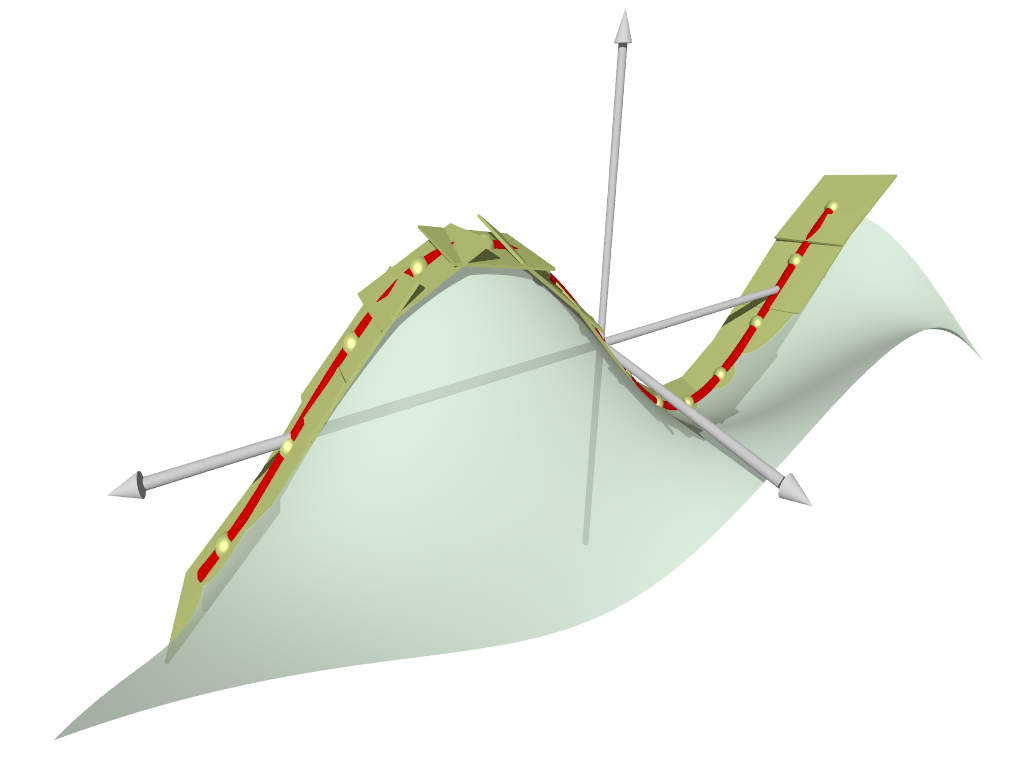
\includegraphics[width=\hsize]{../common/3d/streifen0.png}
\caption{A strip consists of the values and tangent planes
along a curve (red).
The green surface is a solution of the wave equation with the
data of the strip as initial data.
\label{skript:streifen}}
\end{figure}

\begin{figure}
\centering
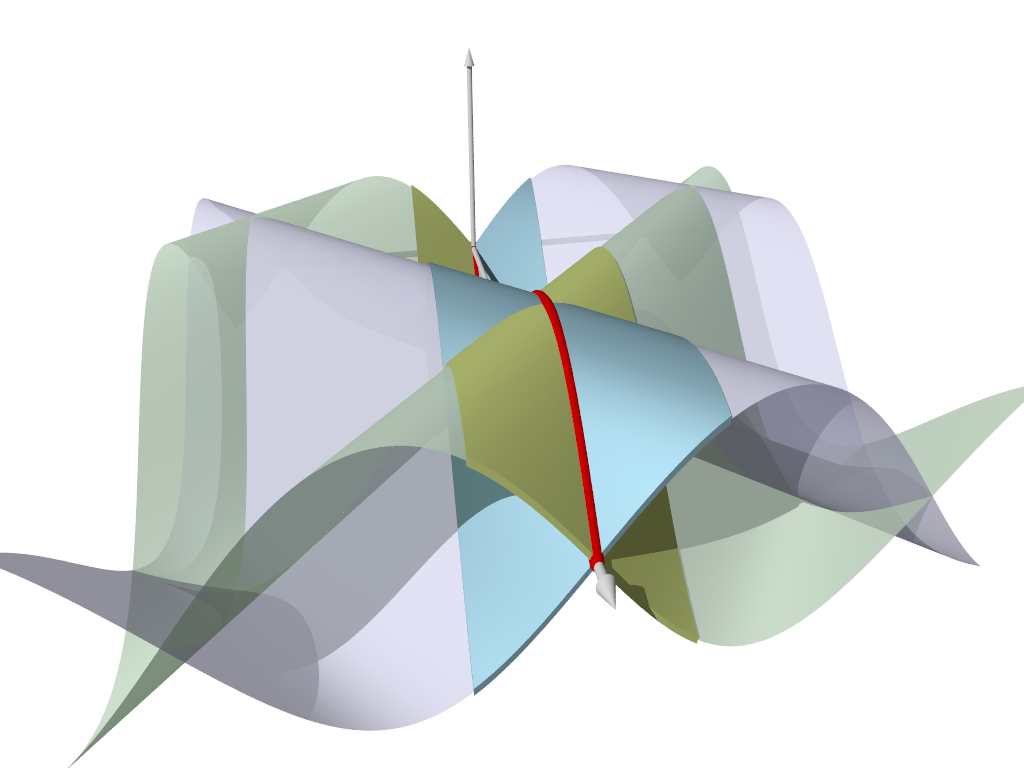
\includegraphics[width=\hsize]{../common/3d/streifen2.png}
\caption{Along the common red curve both solution surfaces have
the same initial values, but different tangent planes, so the
have different strips.
\label{skript:streifen:eindeutig}}
\end{figure}

\begin{figure}
\centering
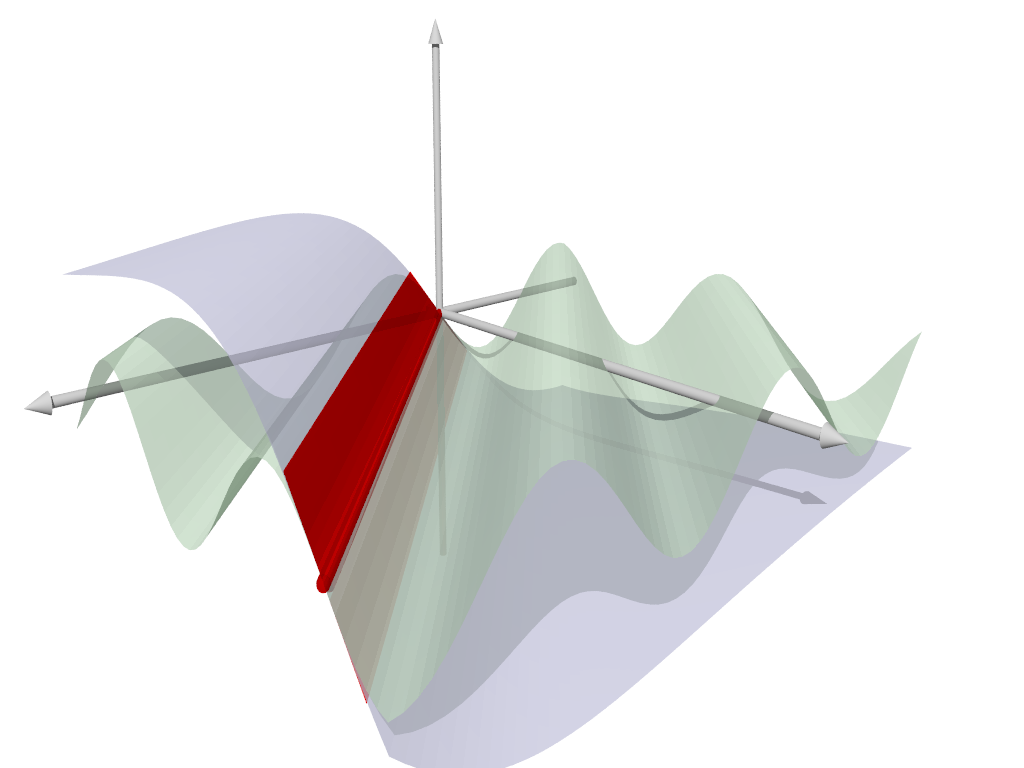
\includegraphics[width=\hsize]{../common/3d/streifen1.png}
\caption{Characteristics are those curves that cannot be used to
define a strip that would uniquely determine the solution surface.
The graph shows two solution of the wave equation with the same
strip: they go through the same curve and they have the same
tangent planes, but the differ in the curvature perpendicular to the
initial curve.
This means that the second order derivatives are not determined by
the equation and the strip data.
\label{skript:streifen:zweideutig}}
\end{figure}

The functions $u(t)$, $p(t)$ and $q(t)$ are not completely arbitrary.
By deriving the first equation \eqref{charanfangs} with respect to $t$,
we find
\[
\dot{u}(t)=\frac{d}{dt}u(t)
=
\frac{d}{dt}u(x(t),y(t))
=
\frac{\partial u}{\partial x}(x(t), y(t))\frac{d}{dt}x(t)
+
\frac{\partial u}{\partial y}(x(t), y(t))\frac{d}{dt}y(t).
\]
Since the partial derivatives are also given in \eqref{charanfangs},
we must also have the relation
\begin{equation}
\dot{u}(t)= p(t)\dot{x}(t) + q(t)\dot{y}(t).
\label{cauchydatarestriction}
\end{equation}

\subsection{Characteristic curves}
Specifying the data of a strip often determines the hyperbolic
partial differential equation uniquely.
In figure~\ref{skript:streifen:eindeutig} two different solutions
are shown that have the same initial curve but different tangent
planes, so the have different strips along this curve.

Deriving the last two equations of \eqref{charanfangs} with respect to $t$,
gives the system of linear equations
\[
\begin{linsys}{3}
\dot p(t)
&=&
\partial_x\partial_xu(x(t),y(t))\,\dot x(t)
&+&
\partial_x\partial_yu(x(t),y(t))\,\dot y(t)
& &
\\
\dot q(t)
&=&
& &
\partial_x\partial_yu(x(t),y(t))\,\dot x(t)
&+&
\partial_y\partial_yu(x(t),y(t))\,\dot y(t)
\end{linsys}
\]
Together with the differential equation we have now three lienar equations
to determine the second partial differential equations:
\[
\begin{linsys}{4}
a{\color{red}\displaystyle\frac{\partial^2 u}{\partial x^2}}
&+&
2b{\color{red}\displaystyle\frac{\partial^2 u}{\partial x\partial y}}
&+&
c{\color{red}\displaystyle\frac{\partial^2 u}{\partial y^2}}
&=&
h(t)
&=&
g-dp(t)-eq(t)-fu\\
\dot x(t)
{\color{red}\displaystyle\frac{\partial^2 u}{\partial x^2}}
&+&
\dot y(t)
{\color{red}\displaystyle\frac{\partial^2 u}{\partial x\partial y}}
& &
&=&
\dot p(t)
& &
\\
& &
\dot x(t)
{\color{red}\displaystyle\frac{\partial^2 u}{\partial x\partial y}}
&+&
\dot y(t)
{\color{red}\displaystyle\frac{\partial^2 u}{\partial y^2}}
&=&
\dot q(t)
& &
\end{linsys}
\]
This linear system of equations for the second order derivatives
has the coefficient matrix
\[
\begin{pmatrix}
a&2b&c\\
\dot x(t)&\dot y(t)&0\\
0&\dot x(t)&\dot y(t)
\end{pmatrix}.
\]
The system of equation is not or not uniquely solvable if the
determinant vanishes, i.~e.
\begin{align*}
0&=\left|\begin{matrix}
a&2b&c\\
\dot x(t)&\dot y(t)&0\\
0&\dot x(t)&\dot y(t)
\end{matrix}\right|
\\
&=a\dot y(t)^2-2b\dot x(t)\dot y(t)+c\dot x(t)^2
\end{align*}

\begin{definition}
The characteristics of a differential equation of the form
\eqref{charequation}
are the curves
$t\mapsto(x(t),y(t))$, for which the initial data 
\eqref{charanfangs} does not determine the second partial
derivatives uniquely.
\end{definition}

\begin{satz}
\label{charakteristikendgl}
The characteristics of a partial differential equation
\eqref{charequation}
solves the differential equation
\[
a\dot y(t)^2-2b\dot x(t)\dot y(t)+c\dot x(t)^2=0.
\]
\end{satz}

\subsection{Characteristic strip}
We shoose a characteristic $t\mapsto(x(t),y(t))$.
We are only interestedin the case where there are infinitely
many possible values for the second derivative.
This case happens when the determinants
\[
\left|
\begin{matrix}
h&2b&c\\
\dot p(t)&\dot y(t)&0\\
\dot q(t)&\dot x(t)&\dot y(t)
\end{matrix}
\right|
,
\quad
\left|
\begin{matrix}
a&h&c\\
\dot x(t)&\dot p(t)&0\\
0&\dot q(t)&\dot y(t)
\end{matrix}
\right|
,
\quad
\left|
\begin{matrix}
a&2b&h\\
\dot x(t)&\dot y(t)&\dot p(t)\\
0&\dot x(t)&\dot q(t)
\end{matrix}
\right|
\]
all vanish, where $h=g-dp(t)-eq(t)-fu(x(t),y(t))$.
It suffices the select a single one of those determinants,
we choose the second:
\begin{align*}
a\dot p(t)\dot y(t)-h\dot x(t)\dot y(t)+c\dot x(t)\dot q(t)&=0
\end{align*}

Together with the condition~\eqref{cauchydatarestriction}
we now have three equations that the functions
$x$, $y$, $u$, $p$ and $q$ must satisfy for the second
derivatives to not be determined uniquely by the initial data.

\begin{definition}
A strip along a characteristic which satisfies
\[
a\dot p(t)\dot y(t)-h\dot x(t)\dot y(t)+c\dot x(t)\dot q(t)=0
\]
is called a {\em characteristic strip}.
\end{definition}

Thus it is also possible, that the integral surfaces of a partial
differential equation touch along a curve, but are different
nevertheless.
By necessity, the tangent planes along the intersection curve form
a characteristic strip.

\begin{satz}
\label{skript:satz:charakteristiken}
If two different integral surfaces touch along a curve,
then this curve together with the tangent planes form a characteristic strip.
\end{satz}

Figure~\ref{skript:streifen:zweideutig} shows two solutions of the wave
equation that touch along a characteristic.
From theorem~\ref{skript:satz:charakteristiken} the red strip is a 
characteristic strip.

\begin{proof}
Apparently there are at least two different solutions of the
partial differential equation that contain the curve which in
addition have the same tangent planes.
The curve and the tangent planes do not determine the solution
uniquely, so the form a characteristic strip.
\end{proof}

\subsection{Examples}
\subsubsection{Wave equation}
The characteristics of the wave equation
\begin{equation}
\partial_t^2u-a^2\partial_x^2u=0
\label{hyperbolisch:wellengleichung}
\end{equation}
are the curves $s\mapsto(t(s),x(s))$, that satisify the equation
\begin{align*}
\left(
\frac{dx(s)}{ds}\right)^2-a^2\left(\frac{dt(s)}{ds}\right)^2&=0
\\
\frac{dx(s)}{ds}
&=
\pm a\frac{dt(s)}{ds}
\\
\Rightarrow
\frac{dx}{dt}=\pm a.
\end{align*}
This are straight lines with slope $\pm a$.
\begin{figure}
\begin{center}
\includegraphics[width=0.8\hsize]{../common/images/char-2.pdf}
\end{center}
\caption{Characteristics of the wave
equation~(\ref{hyperbolisch:wellengleichung})
\label{hyp:wellen}}
\end{figure}
Figure~\ref{hyp:wellen} shows the characteristics.

\subsubsection{The equation $\partial_x\partial_yu=0$}
The condition for the characteristics in this case is
\[
-\dot x(t)\dot y(t)=0
\]
One of the derivatives must disappear, which is only possible for
curves that are parallel to the $x$- or the $y$-axis.
Figure~\ref{hyp:dxdy} shows these characteristics
\begin{figure}
\begin{center}
\includegraphics[width=0.8\hsize]{../common/images/char-3.pdf}
\end{center}
\caption{characteristics of the hyperbolic partial differential equation
$\partial_x\partial_yu=0$.
\label{hyp:dxdy}}
\end{figure}

\subsubsection{Curved characteristics}
The partial differential equation
\begin{equation}
\partial_t^2u-x^2\partial_x^2u=0
\label{hyperbolisch:gekruemmt}
\end{equation}
is hyperbolic for $x\ne 0$.
The characteristics satisfy the equation
\begin{align*}
x'(s)^2-x^2t'(s)^2&=0
\\
xt'&=\pm  x'
\\
\frac{d}{ds}t&=\pm\frac{d}{ds}\log x
\\
t&=\pm\log x+C
\\
x&=x_0e^{\pm t}
\end{align*}
The characteristics are exponential curves.
In figure \ref{hyp:exp}
the characteristics for the positive sign are drawn in red,
the characteristics for the negative sign green.
\begin{figure}
\begin{center}
\includegraphics[width=0.8\hsize]{../common/images/hypexp-1.pdf}
\end{center}
\caption{Characteristics for $x\ne 0$ for the hyperbolic partial
differential equation~\eqref{hyperbolisch:gekruemmt}.
\label{hyp:exp}}
\end{figure}

This equation describes a wave equation in a medium in which
the wave velocity increases with increasing $x$.
The exponential curves suggest that becomes faster when moving ``out''.

\subsection{Characteristics of elliptic or parabolic partial differential
equations}
The theory about the characteristics developed above can also be
applied to elliptic or hyperbolic partial differential equations.

In the elliptic case, the differential equation of the characteristics
\[
a\dot y(t)^2-2b\dot x(t)\dot y(t)+c\dot x(t)^2=0
\]
does not have any solutions, as the expression only vanishes only for
$\dot x(t)=0$ and $\dot y(t)=0$.

For parabolic partial differential equations the characteristic
equation becomes in a suitable coordinate system
\[
-\kappa t'(s)^2=0.
\]
This can only hold true if $t$ is constant.
The characteristics in this case are straight lines parallel
to the $x$-axis.
In fact it is not possible to determine the second derivative
with respect to $t$ for initial data along a line parallel
to the $x$-axis.

\subsection{Some interesting theorems}

\begin{satz}
Every integral surfaces can be covered with a set of characteristic
strips.
\end{satz}

\begin{proof}
Let $u$ be the solution of a partial differential equation.
The differential equation in theorem~\ref{charakteristikendgl}
describes two curves $t\mapsto(x(t),y(t))$ in every point of the domain.
Obviously it is possible to cover the solution surface by such curves.
By substituting these curves into $u(x,y)$, $\partial_xu(x,y)$
and $\partial_yu(x,y)$ we get a set of characteristic strips
as claimed.
\end{proof}

\begin{satz}
If a set of characteristic strips covers a surface $S$ defined
by the function $u(x,y)$ and this function has continuous 
second derivatives then $u$ is a solution of the differential equation.
\end{satz}

\begin{proof}
The characteristic strips satisfy the equations
\begin{equation}
\begin{gathered}
a\dot y(t)^2-2b\dot x(t)\dot y(t)+c\dot x(t)^2=0,
\\
a\dot p(t)\dot y(t)-h\dot x(t)\dot y(t)+c\dot x(t)\dot q(t)=0,
\\
\dot u(t)=p(t)\dot x(t)+q(t)\dot y(t).
\end{gathered}
\label{alle}
\end{equation}
Let's call the second derivatives of $u$ along a cahracteristic curve
\begin{align*}
R&=\partial_x^2u(x(t),y(t)),
\\
S&=\partial_x\partial_yu(x(t),y(t)),
\\
T&=\partial_y^2u(x(t),y(t)),
\end{align*}
We can write
\begin{align*}
\dot p(t)&=R(t)\dot x(t)+S(t)\dot y(t)\qquad\text{and}\\
\dot q(t)&=S(t)\dot x(t)+T(t)\dot y(t)
\end{align*}
If we substitute this in the second equation of \eqref{alle}, then we get
\begin{align*}
a(R\dot x+S\dot y)\dot y-h\dot x\dot y+c\dot x(S\dot x+T\dot y)&=0
\\
\Rightarrow \qquad(aR-h+cT)\dot x\dot y+aS\dot y^2 +cS \dot x^2&=0.
\end{align*}
Multiplying the first equation of
\eqref{alle} by $t$ and subtract it we get
\[
(aR+2bS+cT-h)\dot x\dot y=0.
\]
Writing the parenthesis out is
\[
a\partial_x^2u+2b\partial_x\partial_yu+c\partial_y^2u-h=0
\]
Which is the original differential equation.
\end{proof}
This theorem teaches that the hyperbolic partial differential equation
can be solved by looking for characteristic strips.
for this it suffices the solve ordinary differential equations for the
functions $x$, $y$, $p$, $q$, $R$, $S$ and $T$.


